\section{Logistics}
\label{sec:fdsp-tc-log}


% orig 2nd draft Transporting equipment and people underground is one of the more challenging aspects of the \dword{lbnf}/\dword{dune} endeavor. Access underground goes through the mile long Ross shaft, which is now undergoing renovation. The shaft is outfitted with a single cage for people and materials and two skips that are needed to remove the rock underground. Planning for using the cage is important to making \dword{lbnf}/\dword{dune} a success. Given the enormous cost of the \dword{cf} contracts and the large cost of any inefficiencies in construction, the overall coordinator of the Ross Shaft for \dword{lbnf}/\dword{dune} will be the \dword{cf} \dword{cmgc}. Both \dword{lbnf} and \dword{dune} will also have a large number of contractors, institutions, and scientists who will need to bring equipment and materials underground. \dword{lbnf}/\dword{dune} will establish a logistics organization in South Dakota near \dword{surf} to facilitate the flow of material and people to the underground area. This organization will be responsible for receiving all goods for \dword{lbnf} (except CF) and \dword{dune},for coordinating the transport of this material underground with the \dword{cf}-\dword{cmgc}, and for coordinating personnel usage of the Ross cage with the \dword{cf}-\dword{cmgc}. 

Transport is one of the more challenging aspects of the \dword{lbnf} and \dword{dune} endeavor.  Access to the underground installation area for \dword{lbnf} and \dword{dune} personnel, equipment and materials will be provided by a single shaft, the mile-deep Ross Shaft, which is outfitted with a hoist that controls a cage for transporting people and materials.  
%
Given the enormous cost of the \dword{cf} contracts and the costs of inefficiencies in construction, scheduling use of the shaft is important to making \dword{lbnf} and \dword{dune} successful. A logistics organization is needed to ensure that all deliveries to the Ross Headframe arrive according to schedule. The \dword{lbnf} \dword{cf} \dword{cmgc} will coordinate overall usage of the Ross Shaft for the project. 

\dword{lbnf} and \dword{dune} will establish a logistics organization and lease a warehouse facility within a two-hour drive of  \dword{surf} to facilitate the flow of people and material to the Ross Headframe.  It is expected that this facility, referred to as the \dword{sdwf}, will include warehouse space, personnel and a \dword{wms} system for inventory.  A facility has not yet been selected. 
Most \dword{lbnf} and \dword{dune} material will be shipped to the \dword{sdwf}; \dword{cf} material, and likely cryogenics equipment, are exceptions and will ship directly to \dword{surf}. The logistics  organization will be responsible for (1) receiving and inventorying all  goods shipped to the \dword{sdwf}, and (2) coordinating with the \dword{cf}-\dword{cmgc}  to transport this material to the Ross Headframe in a just-in-time manner. Figure~\ref{fig:logistics-material-flow} shows a high-level overview of the material flow to the Ross Headframe.


%\begin{dunetable}
%[Logistics Specifications]
%{ll}
%{tab:table-Log-Req}
%{Table of logistics specifications.}
%Specifications &  \\ \toprowrule
%Material Handling & Comply with the SURF Material %Handling Specification \\ \colhline
%CMGS coordination & Provide CMGC with two-week notice %of shipments to SURF \\ \colhline
%Stage DUNE Shipments & Provide a one-month local %buffer of DUNE materials \\
%\colhline
%\dword{apa} Storage & Provide storage space for 150 %\dword{apa}s in a clean environment \\
%\colhline
%Inventory & Provide an inventory system accessible to %the collaboration \\
%\end{dunetable}
 %\fixme{Specifications table needs to be converted to official format}
 
% Freight is delivered to the \dword{sdwf}, except for possibly the cryogenic equipment. The materials are then transported in a just-in-time fashion to the Ross headframe where they are brought underground. 
 %For the detector, the \dword{apa}, electronics and \dword{pd} components %will %also be are shipped to the \dword{itf} where they are assembled and then shipped %back  to \dword{sdwf}.
 
\begin{dunefigure}[Material flow diagram for logistics ]{fig:logistics-material-flow}
  {Material flow diagram for the \dword{lbnf} and \dword{dune} logistics.}
 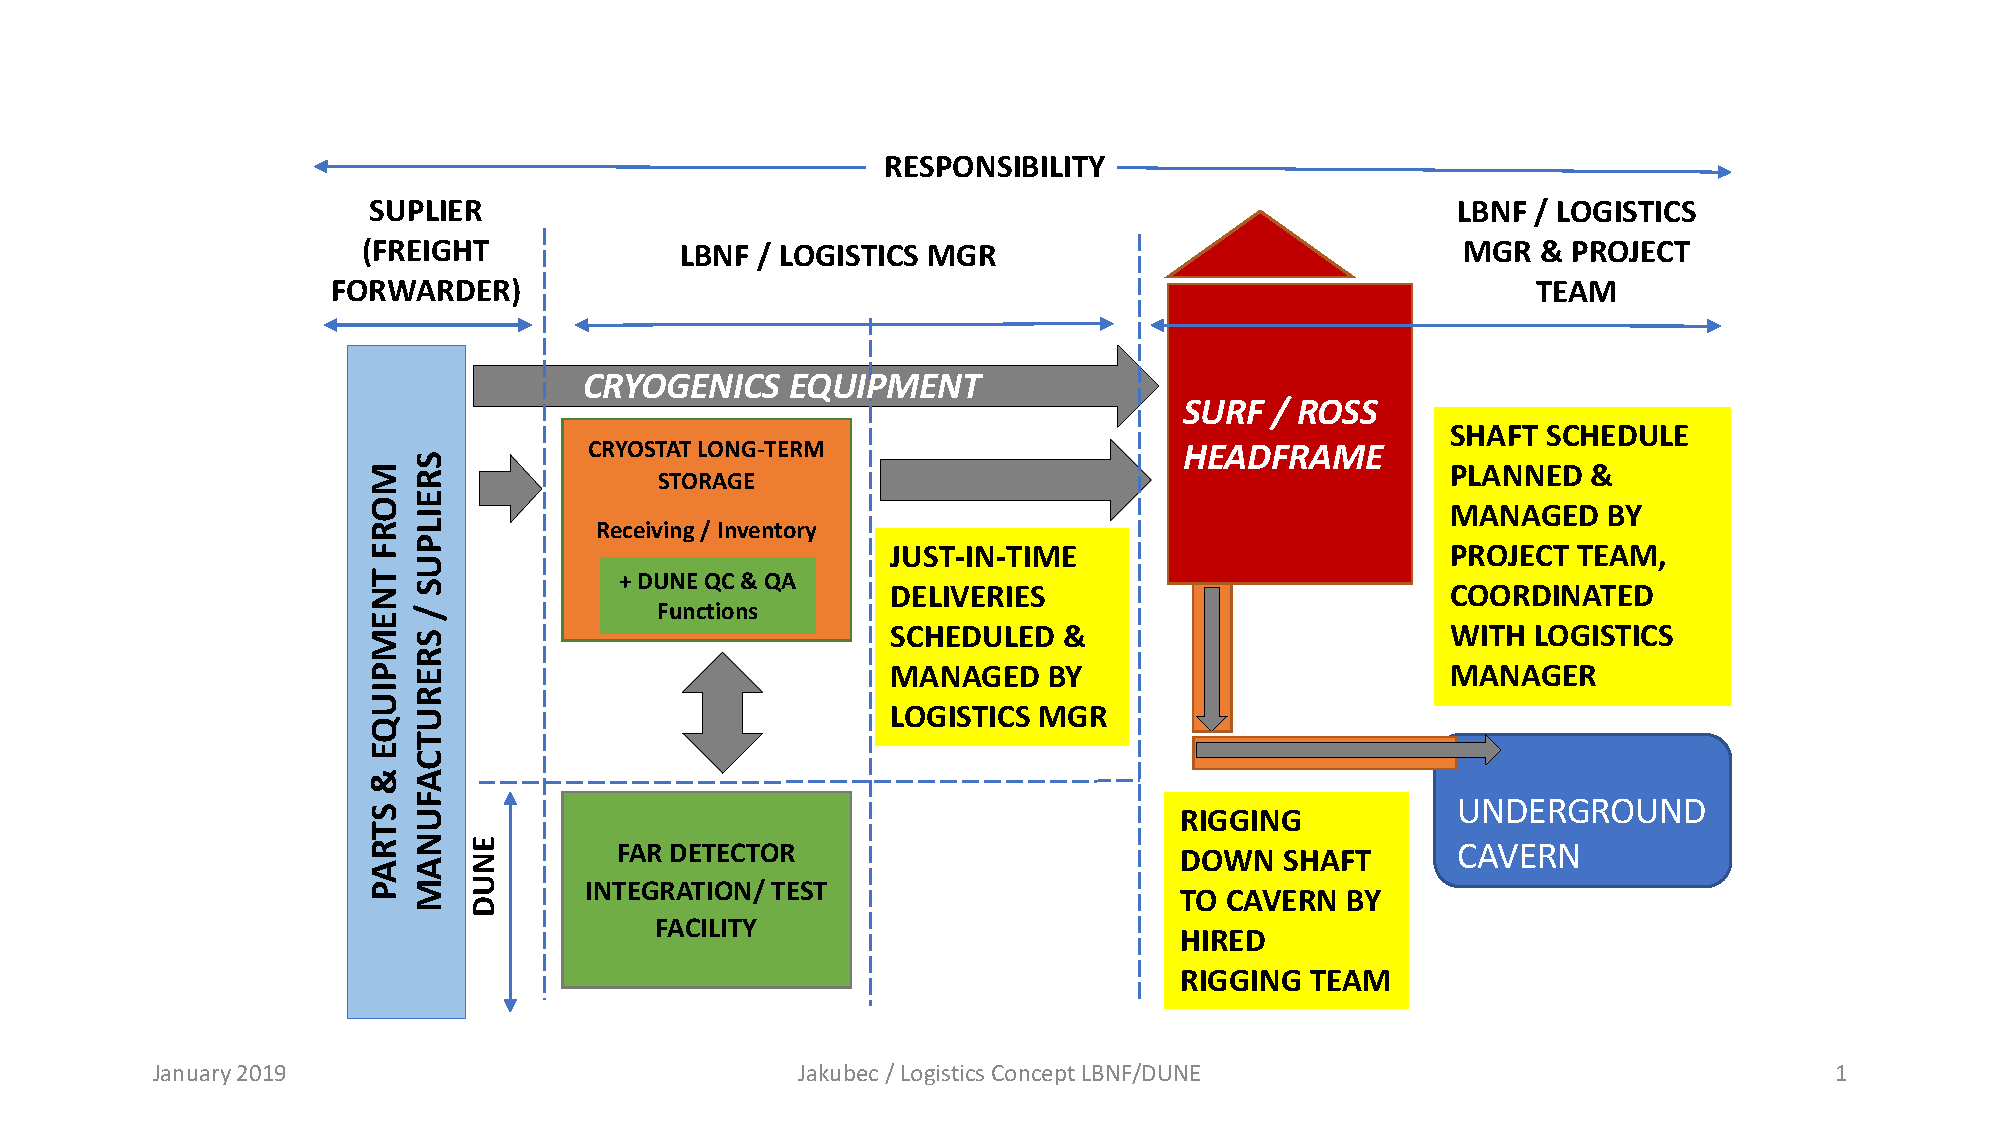
\includegraphics[width=\textwidth]{logistics-material-flow}
\end{dunefigure}

%%%%%%%%%%%%%%%%%%%%%%%%%%%%  
\subsection{Logistics Planning}
\label{sec:fdsp-tc-logPln}

\dword{lbnf} and \dword{dune} logistics oversees transportation of the cryostat (steel, foam, and membrane), the cryogenics system, the detector, and all related infrastructure not provided by %facilities. 
the \dword{cf}. \dword{lbnf} specifically oversees the cryostat and cryogenics system, which %will not be 
are  discussed in detail in %this 
the \dword{lbnf} \dword{tdr}; 
\fixme{add ref} because \dword{lbnf} material dominates the logistics, we present a summary. % is required. 
The %cryostat 
steel structure for each cryostat requires %bringing 
roughly 1,800 individual steel pieces, % underground, 
some of which weigh up to \SI{7.5}{t}, as well as \SI{125}{t} of bolts to assemble the steel pieces. The internal structure for each, which includes the foam insulation and the thin stainless steel membrane, %will 
requires transporting roughly 4,000 boxes, 
 each roughly 1.5 $\times$ 3.5 $\times$ 1.2 m$^3$. The plan for cryostat installation, at present, calls for all components to be warehoused at the \dword{sdwf} before installation begins. %This means that t
This facility will need to have %The logistics operation will  therefore need 
roughly $\SI{5,000}{m^2}$ of  space available to the logistics operation approximately two years before installation of the first \dword{detmodule} begins. By the time detector components start arriving, most of the cryostat boxes will have been removed from the \dword{sdwf}, leaving ample space for the detector and cryogenics components. 
%\fixme{above it says cryogen probably goes straight to headframe???}
Additional space may be required if the boxes for the second cryostat arrive before  \dword{detmodule} \#1 installation is complete; several buildings of the required size are available in the area around \dword{surf}. % if expansion is required.

\begin{dunefigure}
[Simplified model of the Ross Cage]
{fig:fdsp-tc-Cage}
{Simplified Ross Cage model and Specifications.}
\parbox{1.5in}{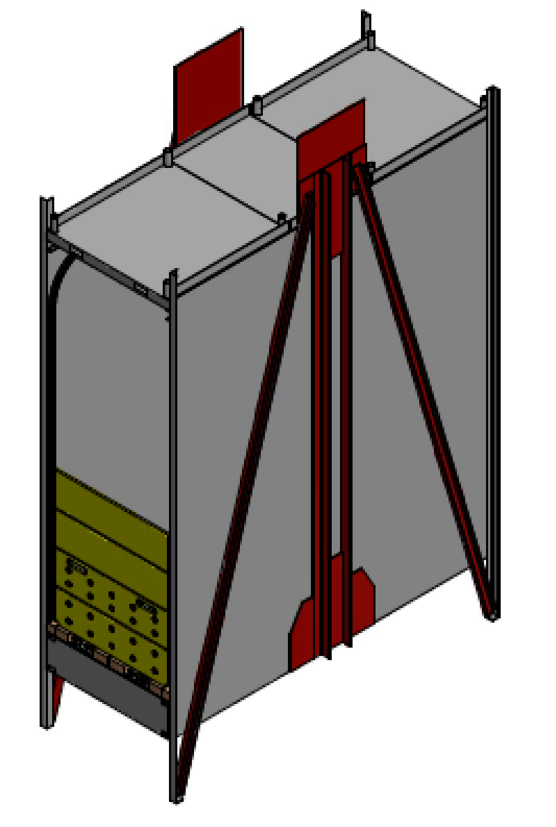
\includegraphics[width=0.32\textwidth]{graphics/Cage-view.pdf}}
\qquad\hspace{60pt}
\begin{minipage}{0.5\textwidth}%
\begin{tabular}{p{3.4cm}p{3.4cm}}        
\multicolumn{2}{c}{Ross Cage Specifications}\\ \toprowrule
Inside height & 3.6 m\\ \colhline
Inside depth  & 3.7 m \\ \colhline
Inside width  & 1.38 m \\ \colhline
Weight limit  &  5,897 kg \\ \colhline
Round trip \newline time & 17 min \newline (incl. unloading) \\ \colhline
\end{tabular}
\end{minipage}
\end{dunefigure}

%All material brought underground must conform to the \dword{surf} Facility Access Specification \cite{bib:docdb328}. This document defines the limitations on dimensions and weights for all materials to be transported underground.  The most important limitations, which are described in detail in the specification document, relate to the Ross shaft and Ross cage. It is possible to bring material down the shaft underneath the cage as a slung load, but this is a much slower process and requires careful planning, detailed procedures, and review. The \dword{dune} \dword{apa}, for example, requires this special handling because they are too tall to fit in the cage. Most material should be brought underground inside the cage. Figure \ref{fig:fdsp-tc-Cage} shows an image of the new Ross cage and Table \ref{tab:table-Ross-Cage} summarizes its parameters. The round trip travel time for the Ross cage is 17 minutes and this is dominated by loading and unloading time. The time needed to load, lower, and unload any slung load is more than an hour round trip as each step is much longer. 
The \dword{surf} Facility Access Specification~\cite{bib:docdb328} defines the limitations on dimensions and weights for all materials to be transported underground, the most stringent of which are set by the Ross shaft and cage. It is possible to bring material down the shaft underneath the cage as a slung load, but this is a much slower process and requires careful planning, detailed procedures, and review. The \dword{dune} \dword{apa}s, for example, require this special handling because they are too tall to fit in the cage. Most material will be brought underground inside the cage. Figure \ref{fig:fdsp-tc-Cage} illustrates the new Ross cage and summarizes its parameters.  The round trip travel time for the Ross cage is 17 minutes (actual travel time is \num{3.6} minutes each way), dominated by loading and unloading time.  Slung loads will require more than an hour round trip.

%\fixme{sorry, I did not keep the orig pgraph here}

The Ross headframe has no loading dock, so careful coordination is required. All materials transported to it must arrive on a flatbed or curtain-sided chassis, where a forklift can unload  the items. The logistics team coordinates all deliveries to the headframe, and the \dword{cf}-\dword{cmgc} coordinates all transport from there down the shaft.  Most material will be delivered first to the \dword{sdwf}, where a central inventory system will capture data about the shipments.  All deliveries, either from this warehouse or direct to the Ross headframe, require (1) coordination with the logistics team, and (2) minimum two weeks prior notice, per an advance delivery plan.  The logistics team will provide a shipping manual \fixme{ref -reserve a docdb?} to \dword{dune} institutions. The institutions must provide shipping data and consign cargo according to the guidelines so that the logistics team can monitor progress. 



In \dword{pdsp}, delays in shipping and customs resulted in up to three weeks delay in the arrival of some parts, which necessitated significant re-planning of the installation work. To prevent this from becoming a much larger problem in \dword{dune}, we plan a minimum one month buffer of materials. This buffer will allow advance planning for the underground work, %can be planned well in advance, knowing 
with confidence that all materials will be available as needed. %This will require that sufficient space be available in the warehouse and underground at \dword{surf} to house the material buffer. Many small parcels will arrive at the warehouse from different sources. 
Sufficient space must be made available in the warehouse and in the underground area  to house this material. % buffer. Many small parcels will arrive at the warehouse from different sources.
The \dword{sdwf} staff will de-consolidate or consolidate arriving cargo into larger boxes and crates, as needed, for  delivery to %the \dword{itf} or 
\dword{surf}, following established % \dword{itf} or \dword{surf} 
delivery plans, to make the most efficient use of available trucks and the Ross Shaft. %hoist. 

\begin{comment}
\end{comment}
\begin{dunefigure}[Underground space needs during installation setup]{fig:fdsp-tc-setup}
  {CAD image showing the empty half of the north cavern as used during the installation setup phase of the first \dword{detmodule}.  Half of this empty space will be used for the cryostat work and half for storage of the detector infrastructure. The material shown outside the cavern must be stored in the \dword{sdwf}.}
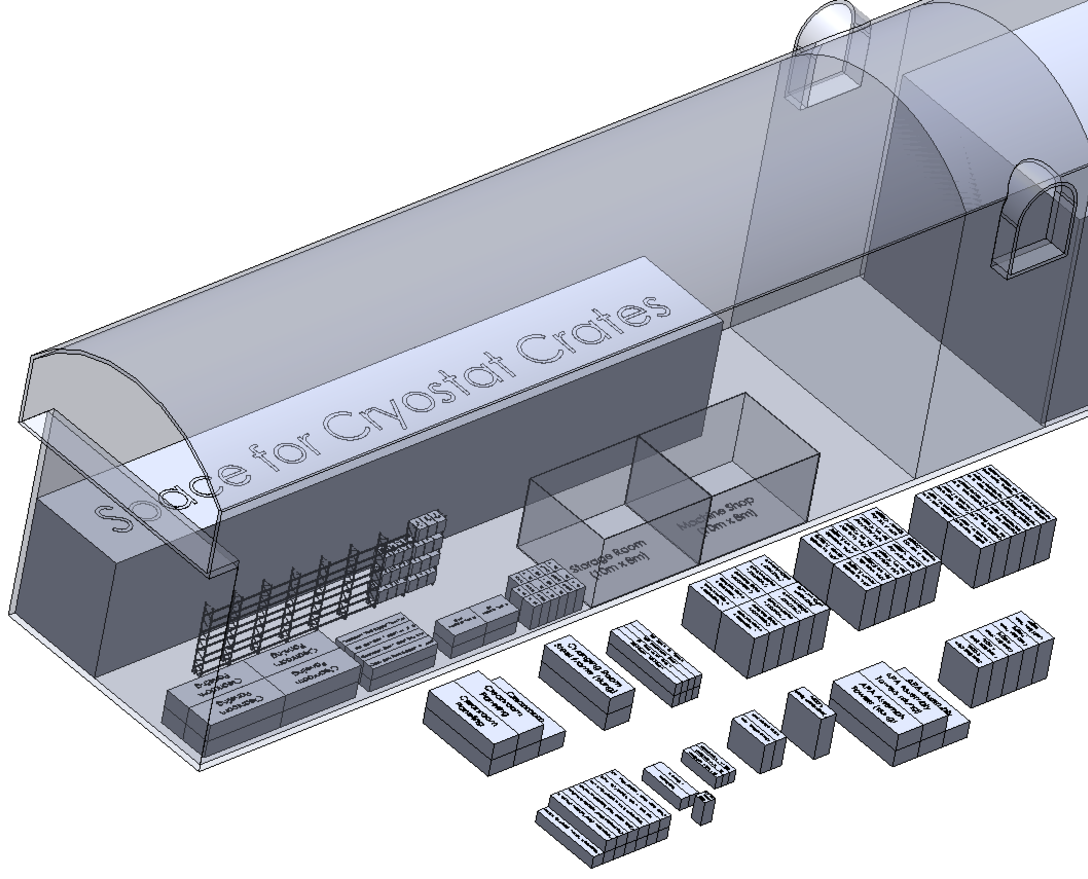
\includegraphics[width=.9\textwidth]{Material-Setup}
\end{dunefigure}


To discover how much space is needed for storage and how much hoist time must be dedicated to \dword{dune}, a detailed inventory of all detector equipment and \dword{dune} infrastructure is needed. The list of %all the 
materials has been solicited from all consortia and technical coordination. The entries in the inventory spreadsheet are organized as ``loads'' for the Ross shaft where a load is a crate or set of boxes that will be transported underground in one trip, either in the %hoist
cage or as a slung load~\cite{bib:docdb8426}. 
Information captured in the load spreadsheet includes the number of %hoist 
trips, type of trip (slung load or cage), package dimensions, weight and type of package (crate, pallet, box, or carton). 

The load list at present predicts 1,600 hoist trips and approximately two  months of cage time, most of which is spread over one year. Installation %operation 
(see Figure \ref{fig:high-level-schedule}) for the \dword{spmod} %detector 
will span two years, so we divide the logistics planning into three  %several 
phases: % is prudent.  The load information is divided into 
(1) the \dword{cuc} setup phase, (2) the installation setup phase, and (3) the detector installation phase. For each phase, a model was generated to show how much material can be stored underground outside the work area and how much material must be stored on the surface. These models set the space requirements for the logistics on the surface. The phase with the largest amount of material to transport is the installation setup phase.  Figure \ref{fig:fdsp-tc-setup} shows the model of the underground area and the required boxes for surface storage for the first third of the setup. This represents the first month of installation setup and shows that roughly 1,000 m$^2$ of warehouse space will be needed for \dword{dune} at this time.  The %warehouse 
\dword{sdwf} will also need space to store up to 150 \dwords{apa}, %in addition to the space needed to receive and ship equipment underground. This 
adding %an additional 
700 m$^2$ to the 1,000 m$^2$. %\ to needed warehouse area. 


%%%%%%%%%%%%%%%%%%%%%%%%%%%%
%\subsection{Logistics Quality Assurance and Quality Control}
\subsection{Logistics Quality Control}
\label{sec:fdsp-tc-log-qaqc}


%\dword{protodune} was an extremely useful exercise in general, but we can draw only a few conclusions about \dword{dune} logistics %because 
%since shipping to Europe differs from shipping to South Dakota and different staff will be responsible for receiving and transport. %the CERN receiving and transport divisions will not be used for \dword{dune}. 
The \dword{protodune} experience offers a couple of significant lessons regarding logistics.

%The full list of %lessons learned is found in the 
%ProtoDUNE-SP lessons learned is in~\cite{bib:docdb8255}. %spreadsheets. 
%The most important lessons learned from \dword{protodune} logistics are: % listed below.
\begin{enumerate}
%\item Lack of a central inventory system made it impossible to track shipments.
%\item Delays in shipping meant that the installation work could not be planned and parts were installed as they arrived. 
\item A central inventory system is essential for tracking  shipments.
\item It is important to avoid delays in shipping because they prevent installation work from  proceeding as planned. 
\end{enumerate}

%To address these issues, a central inventory system will be implemented at the logistics warehouse facility, and a minimum one month material buffer will be required from the consortia in South Dakota.
The central inventory system  implemented at the \dword{sdwf}  and the minimum one-month material buffer are the plans we have in place to prevent repetition of the schedule problems we experienced with \dword{pdsp}.   The full list of lessons learned from \dword{pdsp} is in~\cite{bib:docdb8255}. 

We do not foresee any component testing at the \dword{sdwf}, %in the warehouse, 
so the scope of the \dword{qc} work there is limited to two functions: %A \dword{qa}/\dword{qc} component, however, will be required at receiving. 
%However, a critical \dword{qc} check there %at the logistics facility 
%will 
The facility will ensure that all materials %to be shipped to the Ross headframe 
will fit in the Ross cage, or %. Moreover, 
if a slung load is needed, %the facility will confirm 
that the necessary procedures are in place and approved before any material is transported to the Ross headframe. % to \dword{surf}. 
It will also %The other primary \dword{qc} function performed at the logistics facility is to 
inventory all received shipments. % described below.

%The contribution in kind model of this project makes logistics and inventory control as well as gathering of the relevant construction data extremely complex. Therefore, the logistics (inventory) control and collection of scientific data  must be controlled by independent systems. 
%The logistics supply chain will be controlled by the contributors' freight forwarding system until supplies arrive at the \dword{sdwf}, which has yet to be defined/established.  \dword{sdwf} will be the ultimate point of capture for all \dword{lbnf}/\dword{dune} parts/equipment except possibly for the cryogenic system, given the contractual requirements. The inventory process at the \dword{sdwf}, the \dword{itf} and the \dword{surf} receiving at Ross Shaft will be controlled by one \dword{wms}. 

The contribution-in-kind model of this project complicates logistics, inventory control and the gathering of the relevant construction data. Therefore, the inventory control and the collection of component testing data must be controlled by independent systems. 
Until materials arrive at the \dword{sdwf} or \dword{surf} (if directly shipped), the contributors' freight forwarding system will control the logistics supply chain, which has yet to be defined.  \dword{sdwf} will be the ultimate point of capture for all the materials, except possibly for the cryogenics system, given its special contractual requirements. A central \dword{wms} will control the inventory process at both the \dword{sdwf} and the \dword{surf} receiving at the Ross headframe. 

%The \dword{wms} will provide basic receiving, inventory control, and shipping status for all parts and equipment delivered to \dword{sdwf}. That will include pre-assembled equipment, which will enter as new parts from \dword{itf} as created by the integration work. The \dword{qc}/\dword{qa}, manufacturing, and other relevant data required by the \dword{dune} collaborators will be stored in a separate, as yet undefined and undeveloped, \dword{dcdb}.  The \dword{dcdb} is independent of the \dword{wms} system, and the relevant contributing consortia are responsible for transferring the required data before shipment from supplier to the \dword{dcdb}.  The \dword{wms} database will provide the relevant logistics data to the \dword{dcdb}. The form of data transfer is not yet determined. All \dword{qc}/\dword{qa}, test, and other relevant manufacturing data will be directly input into \dword{dcdb} and will be the responsibility of the different contributing consortia. \dword{dune} must provide a \dword{qc}/\dword{qa} process for all parts/equipment received at the warehouse after being inventoried. That \dword{qc}/\dword{qa} data must be transferred directly to \dword{dcdb} by \dword{dune}.  The \dword{dcdb} will be an integral part of the logistics, assembly, and \dword{qc}/\dword{qa} system. It must provide the \dword{itf} shipping (supply) and assembly reports and create the new equipment denomination for the \dword{wms} to register.  The \dword{dcdb} will document the \dword{itf} sub-assembly process in its entirety.
The \dword{wms} will control basic receiving, inventory control, and shipping status for all components, parts, and equipment delivered to the \dword{sdwf}.  %including equipment  pre-assembled at the \dword{itf}, 
\fixme{I think we don't need anymore: ``which will be entered  as new parts created by the integration work.''} The \dword{qc},  manufacturing, and other %relevant 
data required by the \dword{dune} collaborators will be stored in a separate  %and undeveloped, 
\dword{dcdb} (the system is not yet determined).  


The \dword{dcdb} will be an integral part of the logistics, assembly, and \dword{qc} system.% It must provide the shipping (supply) %and assembly reports and create the new equipment denomination for the \dword{wms} to register.  The \dword{dcdb} will document the \dword{itf} sub-assembly process in its entirety. 
This database will contain all information that needs to be archived, including the shipping reports. 

The consortia are responsible for entering all \dword{qc},  %dword{qa}, 
test, and %other 
relevant manufacturing data directly into \dword{dcdb}.  The \dword{wms} database (available only during the period that we lease the \dword{sdwf}) will provide the associated logistics data to the \dword{dcdb} (the form of data transfer is not yet determined).  The \dword{qc} and shipping data flow is shown in Figure~\ref{fig:logistics-data-and-mat-flow}.

\dword{dune} must provide a post-inventory \dword{qc} %/\dword{qa} 
process to follow for all %parts and equipment 
items at the \dword{sdwf}. 
\fixme{Who at the warehouse executes the QC and adds the data to the DCDB?}

\begin{dunefigure}[QC and shipping data flow diagram for logistics ]{fig:logistics-data-and-mat-flow}
  {QC and shipping data flow diagram for the \dword{lbnf} and \dword{dune} logistics.}
 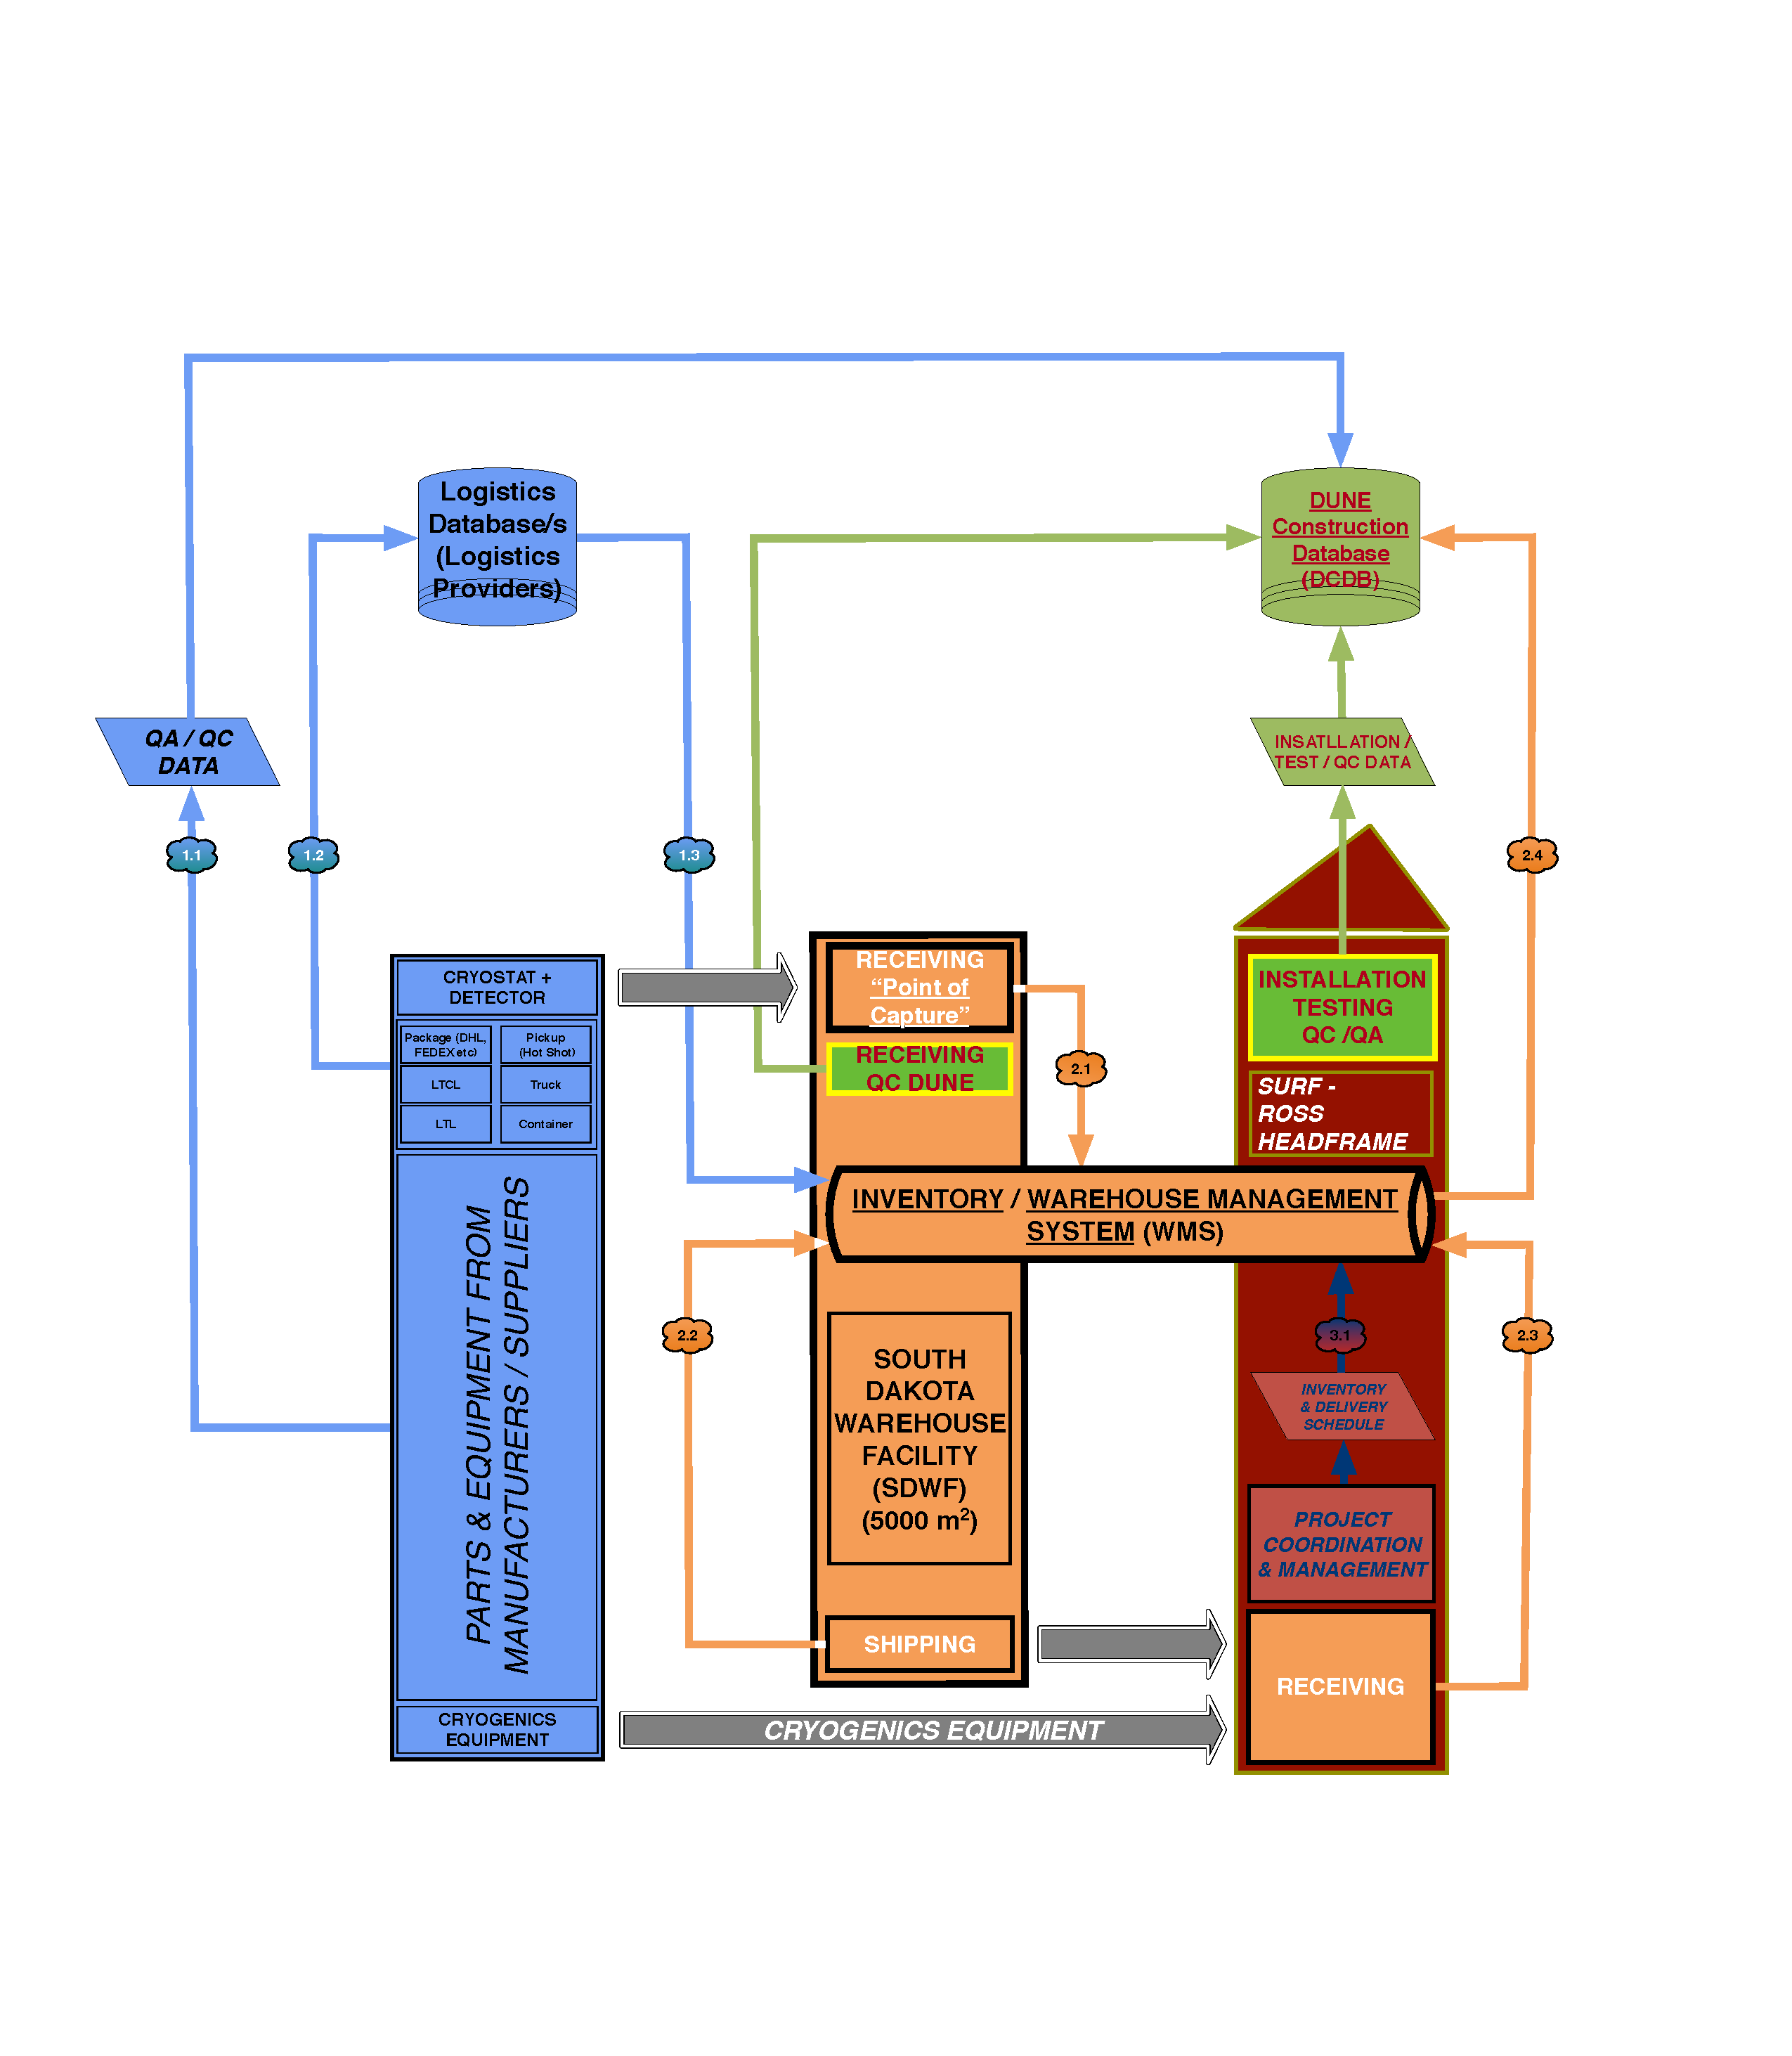
\includegraphics[width=\textwidth]{logistics-data-and-mat-flow}
\end{dunefigure}

%The new sub-assembled items will be inventoried in \dword{wms} as new items during the warehouse receiving process. 
The \dword{jpo} installation management team will provide %be responsible for providing 
a shipping (supply) report to the \dword{sdwf} %for scheduling of 
to schedule each shipment of parts and equipment to \dword{surf}. 
These shipments %from \dword{sdwf} to \dword{surf} 
will be inventoried upon receipt %as received 
at the Ross headframe %\dword{surf} 
in the \dword{wms}. 
Once the items are underground, the \dword{dune} installation team has the responsibility to  %must transfer 
input their % relevant 
\dword{qc}, %/\dword{qa}, 
test, and installation status data to the \dword{dcdb}. % directly.

\fixme{This looks like a summary of the use of the WMS, and it doesn't seem complete. Can we just end this section here, and drop the rest? Anne} To capture all relevant construction and logistics data on parts and equipment, logistics information will %should 
follow this process:

\begin{itemize}
\item The consortia enter data related to %any 
shipments to the \dword{sdwf} into the \dword{wms}. 
\item \fixme{missing the sdwf step}
\item The receiving team at \dword{surf} inventories the shipments from \dword{sdwf} % to  \dword{surf} will be inventoried as received at \dword{surf} 
in the \dword{wms}. The \dword{cmgc}, \dword{lbnf}, \dword{sdsd}, and \dword{dune} will hand off this responsibility among one another at different stages of construction. 
\item Two weeks in advance of any shipment to the Ross headframe, the \dword{jpo} installation management team %will be responsible for 
provides a %shipping (supply) 
report to the \dword{sdwf} detailing the items to ship. %   for scheduling shipments %of parts/equipment to \dword{surf} .
\end{itemize}
\fixme{anne 3/14 - check item 3 above -correct?}

%%%%%%%%%%%%%%%%%%%%%%%%%%%%
\subsection{Logistics Safety}
\label{sec:fdsp-tc-log-safety}

\fixme{talk with Mike A, Niehoff, Bill Miller}

%The \dword{lbnf}/\dword{dune} logistics facility is operated by \dword{sdsd}  as a Fermilab facility, but because of the international connections, we also follow CERN HSE, Fermilab ES\&H, and \dword{surf} ES\&H regulations.  Work is in progress to combine the three into a coherent list of codes and requirements. The \dword{dune} Project ES\&H Coordinator has overall ES\&H oversight responsibility for the \dword{dune} Project.  This person coordinates any activities and facilitates the resolution of any issues that cut across various divisions and institutions and subject to the requirements of the \dword{doe} Workers Safety and Health Program, Title 10, Code Federal Regulations (CRF) Part 851 (10 CFR 851). These requirements are promulgated through the Fermilab Directors Policy Manual and Fermilab ES\&H manual (FESHM), which align with the \dword{surf} ES\&H Manual.  Using the NOvA Far Detector Laboratory as a guideline for remote facilities, several other key documents guide the Logistics Center Safety Program.  The Building Safety Plan combines all building specific documents in a single folder:
The \dword{sdwf}  is operated by \dword{sdsd}  as a Fermilab facility, but because of the international collaboration, we  follow \dword{esh} regulations from CERN and \dword{surf} in addition to Fermilab's.  Work is in progress to combine the three into a coherent list of codes and requirements. The \dword{dune} Project \dword{esh} Coordinator has overall \dword{esh} oversight responsibility for the \dword{dune} Project.  This person coordinates any \dword{esh} activities and facilitates the resolution of any issues that are subject to the requirements of the \dword{doe} Workers Safety and Health Program, Title 10, Code Federal Regulations (CRF) Part 851 (10 CFR 851), and that cut across various divisions \fixme{divisions of what?} and institutions. These requirements are promulgated through the Fermilab Director's Policy Manual \fixme{ref} and Fermilab \dword{esh} manual (FESHM\cite{feshm}), which aligns with the \dword{surf} \dword{esh} manual.  Using the \dword{nova} Far Detector Laboratory as a guideline for remote facilities, several other key documents guide the Logistics Center Safety Program.  The Building Safety Plan \fixme{ref} combines all building specific documents in a single folder:

\begin{enumerate}
\item	Fire Safety and Building Emergency Evacuation Plan, which includes the fire evacuation plan, fire safety plan,  lockdown plans, and the site plan;
\item	Hazard Analysis document, which describes all typical hazards and their mediation %including 
procedures; 
\item	%SDS: 
Safety Data Sheets (SDS), 
\item	Respiratory Plan, as required for chemical or ODH hazards, and 
\item	Training Program, which covers required certifications and  training records.
\end{enumerate}

The current Technical Coordination Facilities Management Plan \fixme{ref} specifies a joint safety officer for %both 
the \dword{itf} and logistics facilities. \fixme{ no ITF, how to rewrite?}This safety officer facilitates training, writes hazard analysis documents, runs weekly safety meetings, and keeps documentation records on materials-handling equipment and personnel. \fixme{what aspect of personnel? sounds a bit 1984ish. }




%%%%%%%%%%%%%%%%%%%%%%%%%%%%
\subsection{Cost and Schedule} %, and Risk Analysis}
\label{sec:fdsp-tc-log-cost}

The costs for the logistics activities and facilities are the responsibility of \dword{lbnf} and Fermilab's \dword{sdsd}, and therefore are not listed here. %  is not a DUNE responsibility and will be covered as part of the host laboratory responsibilities.

According to the overall \dword{lbnf} and \dword{dune} schedule, the \dword{aup} for \dword{lbnf} (post-\dword{cf}) and \dword{dune} teams to the north cavern and \dword{cuc} is \cucbenocc{}.

The  \dword{sdwf} will be in place approximately one year before the warm structure installation begins, i.e., in fall 2021.  Extra storage must be available before  this facility is ready  since  \dword{apa}s, \dword{cuc} infrastructure, and equipment all begin arriving in South Dakota during summer 2021.  As an interim solution, we plan to store these early items at \dword{fnal} until the \dword{sdwf} is ready.

Figure \ref{fig:high-level-schedule} shows the overview of the schedule for the main activities for \dword{detmodule} \#1. 



